\documentclass[12pt]{article}

\usepackage[letterpaper, margin = 1in]{geometry}
\usepackage{fancyhdr}
\usepackage{titling}
\usepackage{titlesec}
\usepackage{hyperref}
\usepackage{lastpage}
%\usepackage{lipsum}
\usepackage{amssymb}
\usepackage{setspace}
\usepackage{stmaryrd}
\usepackage{expex}
\usepackage{tikz}

%%% layout
\usepackage[hmargin=1in,vmargin=0.75in]{geometry}
\usepackage{enumitem}

\usepackage{tabularx}
\usepackage{hanging}

%%% for math
\usepackage{mathtools, amssymb, stmaryrd}
\usepackage{delimset}
  % expanding parens: (  )
  \newcommand{\p}[1]{\brk*{#1}}
  % expanding denotation brackets: [[  ]]
  \newcommand{\sv}[1]{\delim{\llbracket}{\rrbracket}*{#1}}
  % if putting a tree in brackets, the tree must be re-centered, or else the
  % brackets will stretch symmetrically above and below the baseline anchor (the root by default)
  \newcommand{\svtree}[1]{\sv{\vcenter{\hbox{#1}}}}

%%% font stuff
%\usepackage{libertine}
\usepackage{zi4}
\usepackage[dvipsnames]{xcolor}
  \colorlet{tycolor}{Cyan}
  \colorlet{dncolor}{Red}

%%% trees
\usepackage[linguistics,edges]{forest}
  \forestset{%
    default preamble={% this makes all the edges straight
      for tree={% and steamrolls through empty nonterminals
        l=0pt,
        calign=fixed edge angles,
        calign angle=60,
        delay={if content={}{%
          for current and siblings={anchor=north},
          inner sep=0pt,
          edge path={%
            \noexpand\path[\forestoption{edge}]
            (!u.parent anchor) -- (.children) \forestoption{edge label};
          }
        }{}}
      }
    },
  }
  \tikzset{% convenience path for adding movement arrows
    label distance=3pt,
    mv/.style={to path={-- ++(0,-{#1}) -| (\tikztotarget)}},
    mv/.default=0.2
  }

\lingset{
    %aboveglftskip=-1.25em,
    belowglpreambleskip=0pt,
    everyglpreamble=\it,
    everygla={},
    %aboveexskip=0.1ex,
    %belowexskip=0.1ex,
    interpartskip=0em,
    numoffset=1em,
    Everyex=\onehalfspacing
    }

%%% some little macros
% formula stuff
\newcommand{\lam}{\lambda}
\newcommand{\ty}[1]{\texttt{\color{cyan} #1}}
\newcommand{\dt}{{.}\mkern\thinmuskip}
\newcommand{\func}[1]{\textbf{\textsf{#1}}}
\newcommand{\name}[1]{\textbf{\textsf{#1}}}

% tree stuff
\newcommand{\trace}[1]{\texttt{\_\_$_{#1}$}}
\newcommand{\pro}[1]{\text{pro$_{#1}$}}
\newcommand{\pabs}[2][]{\ensuremath{#2_{#1}}}
\newcommand{\remap}[2]{\ensuremath{[#1 \mapsto #2]}}

%%% your task
\newcommand{\FILLIN}[1][dncolor]{%
  {\color{#1}%
    \begin{tabular}{p{1in}}
      \hline\strut\\\hline
    \end{tabular}}}

\usepackage{graphicx}
\graphicspath{ {./images/} }
    
\title{Barker, Bernadi, Shan (2010): \\ Principles of Interdimensional Meaning Interaction}
\author{Ian Thomas White}
\date{}

%\usepackage[backend=biber, style=apa]{biblatex}
%\setlength{\bibhang}{0.5in}
%\addbibresource{201c.bib}
\usepackage{csquotes}
%\DeclareLanguageMapping{english}{english-apa}


\makeatletter
\renewcommand{\maketitle}
{
\begin{flushleft}
\textbf{{\large\@title}}
\newline
\@author
\end{flushleft}
}
\makeatother

\titleformat*{\section}{\medium\bfseries}
\titleformat*{\subsection}{\small\bfseries}

\newcommand*{\textsup}[1]{\ensuremath{^\textrm{{\scriptsize #1}}}}
\newcommand*{\textsub}[1]{\ensuremath{_\textrm{{\scriptsize #1}}}}
\newcommand*{\tinytextsup}[1]{\ensuremath{^\textrm{{\tiny #1}}}}
\newcommand*{\tinytextsub}[1]{\ensuremath{_\textrm{{\tiny #1}}}}

\pagestyle{fancy}
\fancyhf{}
\lhead{Ian Thomas White}
\chead{}
\rhead{\thepage \ of \pageref{LastPage}}

% \linespread{1.6}
\widowpenalty=100000
\clubpenalty=100000

\renewcommand{\labelenumi}{\fbox{\Roman{enumi}}}
\renewcommand{\labelenumii}{\fbox{\Alph{enumii}}}
\renewcommand{\labelenumiii}{\fbox{\roman{enumiii}}}


\begin{document}

\thispagestyle{empty}
\maketitle

\section{Intro}

Side-issue entailments seem to operate in a different realm than at-issue entailments: the former are unable to be modified by any surrounding semantic material. This fact poses an acute problem for compositional semantics, as side-issue entailments are by no means marginal. This means that compositionally accounting for, or at least explicitly rejecting as such, side-issue entailments is not a marginal task but a constitutive problem for a compositional semantics. Barker, Bernadi, \& Shan (2010) take up this task and propose a means for accounting for side-issue entailments in a compositional way. Their analysis relies crucially on undelimited continuations, denotations that are defined ove the semantic context, to analogize side-issue entailments to indexicals.

The present paper essentially follows the logic of the Barker, Bernadi \& Shan paper (henceforth, BBS). Section 1 discusses some empirical facts about side-issue entailments. Section 3 gives a brief overview of two former accounts that treat side-issue content. Section analogizes side-issue content to indexicals. Section 5 presents the computational framework that BBS use for their proposal, the latter of which is described in in section 6. Finally, section 7 discusses some outstanding issues, and section 8 concludes the paper.

\section{At-Issue versus Side-Issue Entailments}

The basic, descriptive distinction between at-issue and side-issue entailments is that the former act as ``news'', new information, while the latter are negatively defined as not-at-issue entailments. For BBS, there are two broad types of side-issue entailments: presuppositions and what I will call ``comments'', the latter of which comprises, at least for BBS, supplements, expressives, and epithets. Examples of each of these are in (1) and (2).
    
\ex Ian put his cat in the shower. \\ \textit{presupposition}: Ian has a cat.
\xe

\vspace*{-1em}\pex 
\a Ian, who is bonked, slept. \\ \textit{supplement}: Ian is bonked.
\a Ian put the toner on his goddamn face. \\ \textit{expressive}: BAD (Speaker has a negative opinion about Ian's face.)
\a Ian asked the goon to chill out. \\ \textit{epithet}: The person Ian asked to chill out is a goon.
\xe

BBS are essentially unconcerned with presuppositions in this paper, focusing instead on comments. Therein, they distinguish comments from presuppositions in several key ways. First, comments are always speaker-oriented, and they always describes some aspect of the discourse situation. This claims holds, at least semantically, they claim, but they note that some (in particular) expressives might offer a ``rhetorical'' pragmatic effect that attributes an attitude to some utterance character distinct from the speaker. For example, a sentence like that in (3) might suggest that \textit{Ian}, and not necessarily the speaker, has negative feelings toward the lawn. The semantics of \textit{wretchedass} in (3), though, they claim, is still speaker-oriented.

   
\ex Ian said to me this morning that he hates to mow the wretchedass lawn.
\xe

\noindent This claim seems harder to make for the change to a deictic or pronoun in (4), especially when imagining the speaker, or the addressee, has met Ian but has never seen Ian's lawn.

\ex Ian said to me this morning that he hates to mow that/his wretchedass lawn.
\xe

Second, comments can and must take widest scope; i.e., they take scope at the level of the utterance/speech-act. This leads BBS to discuss what they call the \textit{non-interaction constraint}, which I repeat in (5). This principle further distinguishes comments from presuppositions, as illustrated in (6).

\ex \textit{Principle of non-interaction:} \\ Once launched, side-issue content does not interact with at-issue content.
\xe 

\pex
\a If I had an Arc Vector, I would talk about my Arc Vector. \\ $\neg$presupposition: Speaker owns an Arc Vector.
\a If I hated the Arc Vector, I would talk about the damn Arc Vector. \\ $\checkmark$comment: Speaker feels negative toward the Arc Vector.
\xe
    
In (6a), the consequent clause contains the presupposition that the speaker owns an Arc Vector, but the antecedent clause can ``satisfy'', or block, this presupposition so that the sentence as whole does not presuppose that the speaker owns an Arc Vector. On the other hand, the consequent clause in (6b) presupposes some negative feeling towards the Arc Vector that the antecedent doesn't satsify or block. Sentence (6b) as whole, then, does presuppose some negative feeling of the speaker toward the Arc Vector.

The principle in (5) can be further illustrated by constructing words that can tamper with side-issue entailments. E.g., a word like \textit{negex} in (7a) can be defined as negating an expressive, or \textit{exonly} in (7b) can be defined as a focus marker that converts a side-issue to an at-issue expression.

\pex
\a Ian \textbf{negex} read the damn book. \hfill [polarity reversal] \\ side-issue: Ian feels good about the book
\a Ian \textbf{exonly} read the damn book. \hfill [focus marker] \\ `Ian [the speaker?] feels worked up about only the book.'
\xe

The situation seems slightly more complicated when comparing (8b) to (8a). 

\pex
\a Ian read the wretched book. \\ expressive: `The book is wretched.'
\a Ian read the supposedly wretched book. \\ ?expressive: `The book is wretched.'
\xe

\noindent Namely, (8a) contains an otherwise normal expressive, \textit{wretched}, while (8b) contains the same expressive modified by the doubt-introducing adverb \textit{supposedly}. It's not clear how BBS would handle this situation; there are at least two possible routes. First, \textit{supposedly wretched} could be taken as one expressive, which might mean the speaker is stating a belief about what other people believe. Second, the scope of the expressive \textit{wretched} is modified by \textit{supposedly}. These two options are not mutually exclusive, but it does raise the question as to how side-issues are syntactically marked as constituents, a problem, I think, that BBS' later discussion does not fully address. The example in (8) further relates to the question of speaker orientation, as \textit{supposedly} strongly suggests that the speaker doesn't maintain the main content of the expressive.

BBS do note, or caveat, some possible interactions between at-issue and side-issue content. Comments can depend on at-issue content for their argument, e.g., \textit{Ian} in \textit{that goon Ian} is an argument of the epithet \textit{goon}; the comment has access to the at-issue content. Quantifiers can also take scope over expressions that launch side-issues. However, once the side-issues are composed they can't be modified or embedded. BBS claim that a side-issue ``proceeds ballistically to its target, which is the context within which the entire utterance is situated''. It's worth asking whether indexicals can also take modificational scope over comments, like in (4), above. This would be a natural way to allows comments to be non-speaker-oriented. Compare, for example (4), repeated in (9a), to (9b). In (9a) \textit{his} takes scope over the expressive, while the expressive takes scope over \textit{of his} in (9b). Furthermore, (9b) much more strongly attributes the expressive to the speaker, while (9a), on my reading, attributes the expressive to \textit{Ian}.

\pex 
\a Ian said to me this morning that he hates to mow his wretchedass lawn.
\a Ian said to me this morning that he hates to mow that wretchedass lawn of his.
\xe
 
\section{Prior Accounts}

BBS discuss two then-recent, prior accounts of side-issues: Potts (2005) and Kubota \& Uegaki (2009).\footnote{ In this section BBS say ``Potts (2007)'', but it's clear they mean ``Potts (2005)''.} Potts' account provides an explicit method for computing at-issue and side-issue content. Therein, side-issues are left ``dangling'' during at-issue computation. All side-issues are computed at the very end of the derivation. A toy schematic of the system is givein in (10). Side-issues dangle underneath the uninterpreted $\bullet$, to be later computed, while at-issue content is computed as normal.
    
\ex[numoffset=1em] \textit{schema for Potts (2007)}

\begin{forest}
[A-I$_\textsf{t}$
[\overline{\textrm{A-I}}]
[\overline{\textrm{A-I}} \\ $\bullet$ \\ S-I$_\textsf{t}$
[\overline{\textrm{S-I}}]
[\overline{\textrm{S-I}}
]
]
]
\end{forest}
\xe

\noindent The problem with this system, according to BBS, is that it's not compositional: the side-issue content is computed from deeply embedded constituents rather than from immediate sub-constituents of the sentence. I'll note, also, that it's not clear how the syntax could produce something like a bullet node in the first place, seeing as the structure is defined semantically. Specifically, as (10) indicates, dangling side-issues are of type \textrm{t}, i.e., the type of a sentence. Presumambly, this could be anything, but selection in the syntax still occurs, even for side-issues, over categories, hence the distinction between (11a,b). How certain side-issues gain type \textrm{t} is thus somewhat unclear.

\pex 
\a Ian bribed [Sue, whom I talked to yesterday].
\a *Ian bribed [Sue, I talked to her yesterday].
\xe

The system in Kubota \& Uegaki (2009), on the other hand, is compositional.  Side-issue content is computed in parallel, i.e. separately but simultaneously, with at-issue content. Side-issue content, moreover, takes scope over a special ``Assn (assertion)'' type. While this system is compositional, it cannot (on its own) explain the non-interaction constraint. Nothing prevents there being some expression in the lexicon that can modify this special type, like \textit{negex} above. Of course, Kubota \& Uegaki could stipulate that there is no such lexical modifier, but this would be less desirable than deriving the facts from the system.


\section{Indexicals Analogy}

What BBS want, then, is a system that is both i) compositional and that ii) allows side-issues to exist on a separate plane without contributing to a sentence's meaning. Side-issue content needs access to the utterance level without being tamperable there: a ``rachet mechanism'' is needed to prevent complete propositions from being re-opened and modified.

BBS propose that side-issue content is in some sense analogous to indexicals. That is, indexicals also involve a semantic relationship between a deeply embedded expression and discourse content, and the semantic effect is generally not modified by intervening material. More specifically, indexicals depend on the discourse situation and are insensitive to embeddings, negation, etc. For example, in (12) \textit{Ian}'s belief must always be about whoever the speaker is, even should \textit{Ian} be mistaken about who the identity of that speaker. The indexical is insensitive to tampering.

\ex Ian believes that I am the Arc Vector
\xe

Still, there is an important difference between indexicals and comments. On the one hand, indexicals depend on the discourse context for content, but they don't modify the context. Comments are essentially the opposite: they do not depend on the discourse context, but they modify the context. Quantifiers, though, take scope within a proposition but don't interact with the context at all. These three types of context-interaction are shown in (13).

\ex a. indexicals / b. quantifiers / c. comments

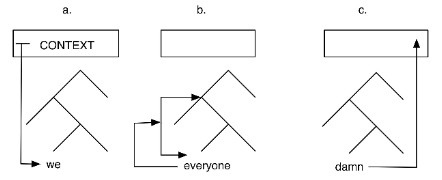
\includegraphics[scale=0.6]{contexts.png}
\xe
    
BBS follow Kaplan in thinkig that context combines with content to determine meaning. Sentences therby denote ``characters'', functions from contexts to contents, meaning the content contains the character, not the indexical. In the course of a derivation, semantic material between the indexical and the utterance level cannot affect the indexical because the indexical has already been replaced by its referent: it's too late for surrounding non-indexical material to modify it.
    
The same idea can be applied to comments. The idea is, again, to use a function from contexts to contents, which is a continuations-passing computation. There are basic two kinds of continuations: i) undelimted (A $\rightarrow \bot$) and ii) delimited (A $\rightarrow$ R$_\signa$). In the former type, $\bot$ is a ``ratchet'', a function that essentially ends a derivation. It thus makes sense to identify ``Assn'' with $\bot$.

\section{Lambek-Grishin Calculus and Continuations}

BBS take the Lambek-Grishin calculus  as their framework for analyzing/computing side-issue entailment. While the actual mechanics are somewhat opaque in this paper, the basic takeaway is that the Lambek-Grishin calculus is a Categorial Grammar, i.e., function application occurs over syntactic categories beefed up with a Logic, i.e., a proof system.\footnote{A constituent is of a certain category iff the cartesian product of its subconstituents form a subset of the category.} Therein,  both expressions and their duals, i.e., contexts, can be precisely calculated. For example, a constituent of type \textit{A}, some structure, can be shown to be parallel to an \textit{A}-type context, a structure with an \textit{A}-hole. This concept is visually represented in (14).

\ex content and context


\includegraphics[scale=0.25]{contents.png}
\xe

\noindent In essence, a structure and its context are symmetrically related. Operators $\backslash , \otimes, \slash $ merge expressions and their duals $\oslash, \oplus, \obslash$ co-merge contexts. Structures and contexts work like the proof in (15).

\pex for structures $\Sigma, \Delta$
\a if $\Sigma \vdash [A\otimes A\backslash B \vdash B]$
\a and if $[B \vdash B \oslahs A \oplus A] \vdash \Delta $
\a then $\Sigma \vdash \Delta$
\xe


Descriptively, (15a) builds a structure B, (15b) builds a stucture context-B, and (15c) ``cuts'' them, i.e., combines them to end the operation. Importantly, for BBS' ratchet-goal, the calculus provides a special type \textit{R}, the result type, which represents a complete derivation (equivalent to $\bot$, above). The Lambek-Grishin calculus thus provides a straightforward way of formulating continuations: the continuation of an expression of Type A is a function from objects of type \textit{A} to \textit{R}.
    
\section{Proposal}

In prior work on Lambek-Grishin continuations, including for purposes of calculating quantifier scope (cf. (13b), above), sentence are of type \textsf{t}, so \textit{R} is of type \textsf{t}. Importantly, expressions don't know that they are type \textsf{t}, quantifiers merely have type \textsf{t} baked into their lexical denotations. BBS, on the otherhand, want to identify \textit{R} with speech acts / utterances, not with propositions. This means \textit{R} must be of a different type than \textsf{t}, the type of a context update.

For determining the type of \textit{R} qua utterance, there are two fundamental facts to be accounted for, as discussed above: i) at-issue and side-issue content contribute to assertions separately; ii) indexicals must have access to the identity of discourse participants. To deal with these facts, BBS start with Murray (2010). For Murray, side-issue content can directly modify the content set in a non-negotiable way; namely, side-issue content removes alternatives from the context set. At-issue content, however, proposes an update to the context set; i.e., it imposes an ordering.

Ultimately, BBS choose a simplification of Murray's system. The context update function returns a pair of propositions of type \textsf{s} $\rightarrow$ \textsf{t}. The first proposition is the set of worlds that  satisfy any background assumptions. The second proposition is the set of worlds that satisfy any at-issue entailments. An addressee can accept at-issue content by taking Prop$_1$ $\cap$ Prop$_2$ or reject at-issue content by taking Prop$_1$ -- Prop$_2$
    
The type of \textit{R}, then, is identified as \textsf{e $\rightarrow$ (s $\rightarrow$ t) $\rightarrow$ ((s \rightarrow t) $\times$ (s $\rightarrow$ t))}: a function from the speaker and an input context set to a pair of propositions. The crux is that indexicals and side-issues can be given different continuized denotations, and these continuized denotations can be defined to take various aspects of the context as arguments. They provide the examples in (16).

\pex 
\a $\llbracket \textrm{my} \rrbracket = \lam \kappa Ps\dt \kappa(\iota x\dt Px \land \func{of}\, s\, x)s$ \\ indexical: (\textsf{e} $\rightarrow$ \textit{R}) $\rightarrow$ ((\textsf{e} $\rightarrow$ \textrm{t}) $\rightarrow \textit{R})$\footnote{The syntactic type they give \textit{my} is \textit{dp/N}, i.e., something that takes takes a noun and produces a DP, so the semantic type here is a function from DP continuations to nominal continuations).}
\a $\llbracket \textrm{damn} \rrbracket = \lam \kappa P s c \dt \langle(\lam w \dt \func{BAD} \, w \land (\pi_1 (\kappa P \, s \, c) w)), \pi_2(\kappa P \, s \, c)\rangle$ \\ expressive: type ((\textsf{e} $\rightarrow$ \textsf{t}) $\rightarrow$ \textit{R}) $\rightarrow$ ((\textsf{e} $\rightarrow$ \textsf{t}) $\rightarrow$ \textit{R})\footnote{The syntactic type they give \textit{damn} is \textit{N/N}, i.e., something that takes takes a noun and produces a noun, so the semantic type here is a function from nominal continuations to nominal continuations).}
\a $\llbracket \textrm{beautiful} \rrbracket = \lam \kappa P \dt \kappa (\func{beautiful}\, P)$ \\ (normal) adjective: type ((\textsf{e} $\rightarrow$ \textsf{t}) $\rightarrow$ \textit{R}) $\rightarrow$ ((\textsf{e} $\rightarrow$ \textsf{t}) $\rightarrow$ \textit{R})
\xe
  
The point is that the indexical in (16a) can take the speaker \textit{s} as an argument such that \textit{s} isn't modified by further computation. For (16b), \textit{s} is again the speaker, and \textit{c} is the context set, and $\pi_1$ and $\pi_2$ return the first and second elements of an ordered pair, respectively. Thus (16b) updates the first proposition set in the context (side-issue content) with the proposition  \fun{BAD}, while the second proposition set (at-issue content) remains unchanged. Note that the normal, i.e., non-expressive, adjective in (16c) has the same type as the expressive in (16b). The crucial difference is that denotations of side-issue content rely on the type of \textit{R} in a way that denotations of at-issue content don't. Namely, at-issue content denotations are \textit{polymorphic} in the result type: they would have the same semantic type regardless of what type \textit{R} is. This is not the case with indexicals and side-issue content because they are lexically defined as taking parts of \textit{R} as arguments. Thus at-issue \textit{beautiful} can't tamper with \textit{damn} once \textit{damn} has been launched.

\section{Remaining Issues}

There are several remaining issues that need to be addressed. First, as BBS themselves note, the system as it stands allows side-issue content to go straight to the utterance level without being tampered with by at-issue content. However, the system doesn't provide generally for the (supposed) inability of side-issue content to tamper with other side-issue content. Of course, it's an empirical question whether or not side-issues can play amongst themselves, separately from at-issue content. Detailing such self-tampering might be a key to dealing with the example from (8b). The more general problem in this vein includes presuppositions. That is, the theory must account for the difference between presuppositions and comments w/r/t the principle of non-interaction (6a,b).

Second, BBS don't explain how expressive vesus non-expressive versions of the same (``same'') word relate, are selected, etc. Presumably the non-expressive \textit{beautiful} from above has an expressive counterpart, akin to \textit{damn}. This distinction would then be encoded in the lexicon, but (how) is the syntax privy to this distinction when building its structures? Furthermore, do we want our lexicon to include a double entry for a large set of words, one entry that's non-expressive and one entry that's expressive (or, more generally, at-issue and side-issue)? In general, how this system interacts with the syntax needs more expression, something the Lambek-Grishin calculus is well equipped to handle. 

Finally, more empirical and theoretical work needs to be done on the question of speaker orientation in comments, as mentioned about (3,4), above. In particular, I think it would be worth exploring the relationship between speakers, as an untamperable fact of the discussion, and the extensions of names. As is commonly assumed, names are considered to have stable extensions across worlds, so I think it would be worth exploring whether side-issue content could compute such extensions directly, or perhaps via indexicals as suggested for (9), above. This might be a way of preserving the major claims of the system in BBS while also allowing more semantic leeway for non-speaker-oriented side-issue content.

\section{Outro}

The present paper has summarized and discussed the main developments from Barker, Bernardi, \& Shan (2010). The basic takeaway is that the difference between side-issue and at-issue content can be treated compositionally and unambiguously in the realm of semantics. To do so the Lambek-Grishin calculus is used to define continuized denotations for side-issue elements that can proceed ``ballistically'' to the level of the utterance. This is an important development towards the goal of systematically integrating otherwise pragmatic phenomena into a compositional semantics.

\section{References}

\begin{hangparas}{.25in}{1}
\small
Barker, Chris, Raffaella Bernardi, \& Chung-chieh Shan. 2010. Principles of interdimensional meaning interaction. In \textit{Semantics and Linguistic Theory} (SALT) 20. 109--127. \url{https://doi.org/10.3765/salt.v20i0.2569}.

Bernardi, Raffaella \& Michael Moortgat. 2010. Continuation semantics for the Lambek-Grishin calculus. \textit{Information and Computation} 208(5). 397--416. \url{https://doi.org/10.1016/j.ic.2009.11.005}.

Kubota, Yusuke \& Wataru Uegaki. 2009. Continuation-based semantics for Conventional Implicatures: The case of Japanese benefactives. In Satoshi Ito \& Ed Cormany (eds.), \textit{Semantics and Linguistic Theory} (SALT) XIX. CLC Publications.

Murray, Sarah E. 2010. A Hamblin Semantics for Evidentials. In Satoshi Ito \& Ed Cormany (eds.), \textit{Semantics and Linguistic Theory} (SALT) XIX. CLC Publications.

Potts, Christopher. 2005. \textit{The Logic of Conventional Implicatures}. Oxford: Oxford University Press.
\end{hangparas}

\end{document}


\begin{tikzpicture}[scale=1]
\draw (0,0) rectangle (0.5,1);
\node at (0.25, -0.25) {A};
\node at (1, 0.5) {$\otimes$};
\draw (1.5,0) rectangle (2,1);
\node at (1.75, -0.25) {A$\backslash$B};
\node at (2.5, 0.5) {$\Rightarrow$};
\draw (3,0) rectangle (4,1);
\node at (3.5, -0.25) {B}
\end{tikzpicture}